\nonstopmode
% \documentclass[11pt,twoside]{article}
\documentclass[11pt]{article}


%%%%%%%%%%%%%%%%%%%%%%%%%%%%%%%%%%%%%%%%%%%% 

% TODO: Wurden alle %todo-Marker bearbeitet?

%%%%%%%%%%%%%%%%%%%%%%%%%%%%%%%%%%%%%%%%%%%% 


\def \GiveSolution {1}
\usepackage{etex} % more counters
\usepackage{a4wide}
\usepackage{fancyhdr}
\usepackage[utf8]{inputenc}
\usepackage{amsthm,amssymb,stmaryrd}
\usepackage{color}
% \usepackage{bcprules}
\usepackage{amsmath}
\usepackage{boxedminipage}
\usepackage{calc}
\usepackage{ifthen}
\usepackage{verbatim}
\usepackage{fancyvrb}
\usepackage{listings}
\usepackage{framed}
\usepackage{graphicx}
\usepackage{dashrule}
\usepackage{multirow}
\usepackage{totcount}
\usepackage{multido}
\usepackage{tikz}
\usepackage{xypic}
\usepackage{xfrac}
\usepackage{dsfont}

\theoremstyle{plain}
\newtheorem{assumption}{Assumption}
\newtheorem{lemma}{Lemma}
\newtheorem{theorem}{Theorem}
\newtheorem{corollary}{Corollary}
\theoremstyle{definition}
\newtheorem{definition}{Definition}
\theoremstyle{remark}
\newtheorem{remark}{Remark}
%\newtheorem{solution}{Solution}



\DeclareSymbolFont{bbold}{U}{bbold}{m}{n}
\DeclareSymbolFontAlphabet{\mathbbold}{bbold}

\newcommand\Reals {{\mathds{R}}}
\newcommand \E {\mathop{\mbox{\ensuremath{\mathbb{E}}}}\nolimits}
\renewcommand \Pr {\mathop{\mbox{\ensuremath{\mathbb{P}}}}\nolimits}


\usetikzlibrary{automata}
\usetikzlibrary{topaths}
\usetikzlibrary{shapes}
\usetikzlibrary{arrows}
\tikzset{
  arn/.style = {circle, draw=black}
}
\usetikzlibrary{decorations.markings}
\usetikzlibrary{intersections}

\tikzstyle{place}=[circle,draw=black,inner sep=0mm, minimum size=6mm]

\tikzstyle{utility}=[diamond,draw=black,draw=blue!50,fill=blue!10,inner sep=0mm, minimum size=8mm]
\tikzstyle{select}=[rectangle,draw=black,draw=blue!50,fill=blue!10,inner sep=0mm, minimum size=6mm]
\tikzstyle{hidden}=[dashed,draw=black,fill=red!10]
\tikzstyle{RV}=[circle,draw=black,draw=blue!50,fill=blue!10,inner sep=0mm, minimum size=6mm]

\tikzstyle{transition}=[rectangle,draw=black!50,fill=black!20,thick]
\tikzstyle{someset}=[circle,draw=black,minimum size=8mm]
\tikzstyle{point}=[circle,draw=black,fill=black]



\renewcommand*\ttdefault{txtt} % for listing package

\parindent0em
\parskip1ex plus0.25ex minus0.25ex

\setlength{\voffset}{-1.6cm}
\setlength{\textheight}{25.5cm}
\setlength{\hoffset}{-5mm}
\setlength{\textwidth}{17cm}


\newcommand{\NN}{\mathbb{N}}
\newcommand{\ZZ}{\mathbb{Z}}
\newcommand{\omod}{\mathrel{\mathrm{mod}}}

\usetikzlibrary{arrows}
\tikzset{
  arn/.style = {circle, draw=black}
}

\renewcommand*\ttdefault{txtt} % for listing package

\parindent0em
\parskip1ex plus0.25ex minus0.25ex

\setlength{\voffset}{-1.6cm}
\setlength{\textheight}{25.5cm}
\setlength{\hoffset}{-5mm}
\setlength{\textwidth}{17cm}


\pagestyle{empty}

\fancyhead{}
\fancyhead[LO]{Written Exam, IN-STK-5000, Autumn 2019}
\fancyhead[RO,RE]{\thepage}
\fancyfoot{}

\RequirePackage{color}
\RequirePackage{boxedminipage}
\RequirePackage{ifthen}
\definecolor{ErrorRed}{rgb}{1,0.80,0.80}
\definecolor{NoteBlue}{rgb}{0.8,0.80,1.0}
\definecolor{CorrectGreen}{rgb}{0.8,1.0,0.8}
\definecolor{ExampleGrey}{rgb}{0.8,0.8,0.8}



\newcommand{\COMMENT}[2][]{$\maltese$\begin{Large}\textbf{COMMENT #1:} #2\end{Large}$\maltese$}

\renewcommand*\ttdefault{txtt}

\newcommand{\blank}[1]{\hdashrule{#1}{1pt}{1pt 4pt}}

\newcommand{\breakpage}{

  \vfill
  
  \hspace*{-4EX}\emph{Continued on next page}
  \vspace*{4EX}
  
  \newpage
  
  \hspace*{-4EX}\emph{Continuation of question~\ref{A\arabic{aufgno}}:}  
} 




\providecommand{\deflistings}[1]{%
  \lstset{%
    language=#1,%
    basicstyle=\small\ttfamily,%
    keywordstyle=\bfseries,%
    identifierstyle=,%
    commentstyle=\itshape,%
    showstringspaces=false,%
    extendedchars=true,%
    escapeinside={/*}{*/}
  }%
}
\deflistings{Java}

%% Markus, 2011-12-13: Added handling of umlauts
%% Source: http://www.artikcommunity.biz/showthread.php?t=10931382#post47117516
\lstset{extendedchars=true,literate={ä}{{\"a}}1 {ö}{{\"o}}1 {ü}{{\"u}}1 {Ä}{{\"A}}1 {Ö}{{\"O}}1 {Ü}{{\"U}}1 {ß}{\ss}1}


%% Markus, 2011-12-13: Added handling for long source lines
%% Source: http://www.ureader.de/message/1543599.aspx
%% Unfortunately \rotatebox seems not to work within ``prebreak''.
%% So we save the the symbol in box in advance.
%% However, rotatebox is not allowed in the preamble
%% (http://newsgroups.derkeiler.com/Archive/Comp/comp.text.tex/2011-01/msg00912.html)
%% Hence, we execute the code at the begin of the document.
\AtBeginDocument{%
  \newbox{\lstbreaksym}%
  \savebox{\lstbreaksym}{\;\raisebox{.9ex}[0ex][0ex]{\rotatebox{180}{\ensuremath{\Rsh}}}}%
  \lstset{
    breakautoindent  = true,
    breakindent      = 2em,
    breaklines       = true,
    postbreak        = ,
    prebreak         = \usebox{\lstbreaksym},
  }%
}
\usepackage{hyperref}


% Automatic Numbering by Steffen 

% Pages
\newcounter{emptypages}
\setcounter{emptypages}{5}
\regtotcounter{page}
\newcounter{adjustedpages}
\newcommand{\updatepages}{\setcounter{adjustedpages}{\totvalue{page}}\addtocounter{adjustedpages}{-\value{emptypages}}}

% Points
\newtotcounter{aufgno}
\newtotcounter{sumpoints}
\newcounter{halfpoints}
\newcommand{\makepcounter}[1]{\newcounter{volatilepoints#1}\newtotcounter{points#1}}
% \multido{\i=1+1}{20}{\makepcounter{\i}} %%% Does not work unfortunately
\makepcounter{1}
\makepcounter{2}
\makepcounter{3}
\makepcounter{4}
\makepcounter{5}
\makepcounter{6}
\makepcounter{7}
\makepcounter{8}
\makepcounter{9}
\makepcounter{10}
\makepcounter{11}
\makepcounter{12}
\makepcounter{13}
\makepcounter{14}
\makepcounter{15}
\makepcounter{16}
\makepcounter{17}
\makepcounter{18}
\makepcounter{19}
\makepcounter{20}
\makepcounter{21}
\makepcounter{22}
\makepcounter{23}
\newcommand{\setpoints}[2]{\setcounter{points#1}{#2}}
\newcommand{\gettotpoints}[1]{\total{points#1}}
\newcommand{\getpoints}[1]{\arabic{volatilepoints#1}} % \gettotpoints{} cannot be used everywhere, hence we need to copy the values into normal counter after begin document
\newcommand{\copypoints}[1]{\setcounter{volatilepoints#1}{\totvalue{points#1}}}
\newcommand{\updatepoints}{%
  \multido{\I=1+1}{\totvalue{aufgno}}{\copypoints{\I}}%
  \setcounter{halfpoints}{(\totvalue{sumpoints}+1)/2}%
}


% \newcommand{\option}{\raisebox{-1.5mm}{\Huge $\Box$}\enspace}


%%% Question
\newenvironment{question}[2]{
  \refstepcounter{aufgno}%
  \setpoints{\arabic{aufgno}}{#2}
  \addtocounter{sumpoints}{#2}%
  {\bf Question~\arabic{aufgno} (#1): \hfill (#2 Point(s))
    \phantomsection\addcontentsline{toc}{chapter}{A\arabic{aufgno} (#2): #1}\label{A\arabic{aufgno}}
    \\[2mm]
  }
}{}

\newenvironment{solution}{\par\textbf{Solution:} }{\qed \par\noindent}






\newcommand{\otto}{\leftrightarrow}


% Logic                         .5 + .5
% (compute value of prop formula)
% give entire truth table
% decide taut/contradiction/equivalence
% deductive proof given equiv and infer rules
% (english sentence)
% (predicate logic)
% Recursion                     .5
% write a recursive program
% (rec sets)
% (single/multiple recursion)
% (compare iteration)
% Induction, Stacks             .5
% (induction)
% (abstract datatypes (interfaces, generics))
% (implement stack)
% (program stack)
% Complexity                    .5
% tell complexity of given program
% (big O notation def, calculation)
% (best/worst case)
% Trees                         1
% (definitions)
% (implementation, array repr)
% (Huffman coding)
% (binary search trees)
% Graphs                        1
% (definitions)
% (euler's theorem)
% adjecency matrices/lists
% dijkstra's
% Sets                          1
% (defs)
% compute sets
% set comprehension
% pairs, tuples
% power sets
% (mappings, functions)
% Sorting                       1
% (orderings, partial/total relations, Hasse diagrams)
% heap sort
% quick sort
% merge sort
% Matrices                      1
% matrix algebra
% Hashtables                    .5
% hash function
% example construct hash table (linear probing, lists)
% total                         8
% 4.5 points per 1 lecture


% Logic
% prop formulas
% thruth tables
% reasoning
% negate english sentence
% quantifiers decide truth
% Graphs
% adjecency matrix/list
% paths, cyclic paths
% Euler paths
% Sets
% set algebra
% power sets
% set comprehension
% projection
% Trees
% def height balanced tree
% pre/in/postorder traversal
% binary search trees insertion, removal
% Hash tables
% store numbers given hash function (linear probing, linked list)
% load factor
% Heap
% definition
% storing as arrays
% insertion/removal
% Sorting
% merge sort
% Complexity
% decide complexity of given code
% give complexity of sorting algs
% Stack
% write a little program
% Matrix algebra
% mult, inverse, vectors
% Recursion
% write a small rec program
% Misc
% dryrun and explain given program


\begin{document}
\updatepoints
\updatepages

EXAMINATION
\\[1cm]
\begin{large}
  \textbf{Adaptive Methods for Data-Based Decision Making (IN-STK 5000/9000), 10 ECTS}
\end{large}
\\[.5cm]
Informatics, Mathematics\\
University of Oslo\\


\begin{tabular}{@{}ll}
  Date & \textbf{N/A} \\
  Results & \textbf{N/A} Solution suggestions on course web page after the exam. \\
  Allowed aids &  Any written or printed material\\
  Exam grade limits & A: 90\%, B: 80\%, C: 60\%, D: 50\%, E: 40\%, F: <40\%.
\end{tabular}

\vspace{1cm}


Please observe the following:
% (failing to do so may result in point deduction):
\begin{itemize}
\item Write in \emph{legible} English (unreadable means
  no points).
\item \textbf{Motivate your answers, explain your calculations, and clearly state any assumptions made. Insufficient justifications will lose points. Questions where no calculations are required are clearly marked.}
\item Questions marked with (*) may require additional thought.
\item  \emph{State clearly to which question each answer belongs.}
\end{itemize}

\begin{large}
  Good Luck!
\end{large}

\vspace{1cm}

\let\NumberCols\empty%
\begingroup%
\multido{\i=1+1}{\totvalue{aufgno}}{\xdef\NumberCols{\NumberCols c|}}%
\endgroup%
\let\NumberRow\empty%
\begingroup%
\multido{\i=1+1}{\totvalue{aufgno}}{ \xdef\NumberRow{\NumberRow\i&}}%
\endgroup%
\let\PointRow\empty%
\begingroup%
\multido{\i=1+1}{\totvalue{aufgno}}{ \xdef\PointRow{\PointRow \getpoints{\i} &}}%
\endgroup%
\newlength{\boxwidth}
\setlength{\boxwidth}{(\linewidth - 18em) / (\totvalue{aufgno}+6) }
\newsavebox{\emptywidth}
\sbox{\emptywidth}{\hspace{\boxwidth}}
\let\EmptyRow\empty%
\begingroup%
\multido{\i=1+1}{\totvalue{aufgno}}{ \xdef\EmptyRow{\EmptyRow\usebox{\emptywidth}&}}%
\endgroup%
\addtolength{\boxwidth}{3mm}

\begin{center}
  \begin{tabular}{|l||\NumberCols|c|c||c|}
    \hline
    \large No.\rule[-2ex]{0em}{6ex}  & \NumberRow $\sum$  & \large Mark \\ \hline
    \large Max \rule[-2ex]{0em}{6ex}   & \PointRow  \textbf{\total{sumpoints}} & \\ \hline
    \large Points\rule[-2ex]{0em}{6ex} & \EmptyRow  \hspace*{\boxwidth} &\hspace*{\boxwidth} \\ \hline
  \end{tabular}
\end{center}


\newpage

% \pagebreak %% bei Option twoside
% \quad      %% bei Oprion twoside
\newpage

%%% END

\parindent0em
\parskip1ex plus0.25ex minus0.25ex

\newenvironment{code}{\begin{quote}\tt}{\end{quote}}

% \newcommand{\bittewenden}{\fancyfoot[R]{-- bitte wenden --}\newpage\fancyfoot{}}
\newcommand{\bittewenden}{\newpage}

\setlength{\voffset}{-1.6cm}
\setlength{\textheight}{25.5cm}
\setlength{\hoffset}{-5mm}
\setlength{\textwidth}{17cm}

\pagestyle{empty}

\fancyhead{}
\fancyhead[LO]{Examination for IN-STK-5000, 2019}
\fancyhead[RO,RE]{\thepage}
\fancyfoot{}
% \cfoot{}

\setcounter{page}{1}
\pagestyle{fancy}

\renewcommand{\theenumi}{\alph{enumi}}
\renewcommand{\labelenumi}{\textbf{\theenumi)}}

\begin{question}{Markov decision processes}{1}
  The following diagram shows a Markov decision process where the circles denote states, the squares denote action notes, and the rhomboids reward nodes. The probability of reaching a state by taking different actions is given on the connecting edges. The process ends after two steps and the utility is defined as the total reward $U_t = r_t + r_{t+1}$. Calculate the expected value of the first state at $s_t$ for the optimal policy, i.e. the one maximising expected utility.

  \centering
  \begin{tikzpicture}
    \node at (0, -3) {$s_t$};
    \node at (2, -3) {$a_t$};
    \node at (3, -3) {$r_t$};
    \node at (5, -3) {$s_{t+1}$};
    \node at (6, -3) {$r_{t+1}$};
    \node[RV] at (0,0) (s1) {};
    \node[select] at (2,-1) (a1) {};
    \node[select] at (2,1) (a2) {};
    \node[utility] at (3,2) (r2) {$1$};
    \node[utility] at (3,-2) (r1) {$0$};
    \node[RV] at (5,1) (s2a) {};
    \node[RV] at (5,-1) (s2b) {};
    \node[utility] at (6,2) (r2a) {$0$};
    \node[utility] at (6,-2) (r2b) {$1$};
    \draw[->] (s1) to node [sloped,anchor=south] { } (a1);
    \draw[->] (s1) to node [sloped,anchor=south] { } (a2);
    \draw[->] (a1) to node [sloped,anchor=north] {$0.2$} (s2a);
    \draw[->] (a1) to node [sloped,auto] {$0.8$} (s2b);
    \draw[->] (a2) to node [sloped,auto] {$0.4$} (s2a);
    \draw[->] (a2) to node [sloped,anchor=east] {$0.6$} (s2b);
    \draw[->] (a1) to (r1);
    \draw[->] (a2) to (r2);
    \draw[->] (s2a) to (r2a);
    \draw[->] (s2b) to (r2b);
  \end{tikzpicture}
  \if \GiveSolution 1
  \begin{solution}
    The top state has value $0$ and the bottom has value $1$.
    Hence the top action has value $0.6 + 1$ and the bottom $0.8$.
    Hence the top action is the best, and the optimal policy chooses it. Then the value of the first state is $1.6$.
  \end{solution}
  \fi
\end{question}


\begin{question}{Simple decision problems}{4}\label{q:probability}
  Consider the following basketball matches. Firstly, a match between Helsinki
  Hippopotami and Gothenburg Geese and secondly a match between the Stockholm Spaniels  and the Oslo Occelots. 


  \begin{enumerate}
  \item Assume that the outcomes of the matches are independent. You estimate that Helsinki has a 60\% chance of beating Gothenburg, so $P(H) = 0.6$ while Stockholm has a 70\% chance of winning over Oslo, so $P(S) = 0.7$.
  There are two bookies, which allow you to bet on the outcome of the matches. The first bookie gives you odds 3/2 that \emph{both Helsinki and Stockholm win}. The second bookie gives you odds 2/1 for a Helsinkini and Stockholm win.
  (An odds of 3/2 for an event means that you gain 3 NOK for each 2 NOK you bet if the event occurs. So if you bet that \emph{both Helsinki and Stockholm win} with the \emph{first} bookie, and they do, then you get your 1 NOK back and you also gain 3/2 = 1.5 NOK. Similarly, you can gain 2 NOK if you place the same bet with the second bookie and you win.)
    Given your assumptions, which of the two bookies gives you the highest expected amount of money for the bet that Helsinki and Stockholm both win? Show your calculations in detail.
    \if \GiveSolution 1
    \begin{solution}
      First of all, the chance of the bet comes off is $P(H S) = P(H) P(S) = 0.42$ due to independence. The expected gain in the first case is
      \[
      1.5 \cdot P(H S) - 1 \cdot (1 - P(HS)) = 0.63 - 0.68 = -0.65
      \]
      In the second case, it is
      \[
      2 \cdot P(H S) - 1 \cdot (1 - P(HS)) = 0.84 - 0.68 = 0.16
      \]
      So it is obviously better to take the second bookie's offer if you want to maximise expected money gain.
    \end{solution}
    \fi
  \item However, you realise that the Stockholm match is after the Gothenburg match. Due to well-known problems with corruption in sports, there is then a chance that Stockholm would be bribed into losing too, since the match would not be important to them anymore. Specifically, you guess that if Gothenburg loses, then Stockholm has a lower chance of winning: 50\%, i.e. that $P(S \mid H) = 0.5$. However, if Gothenburg wins, then you still estimate that Stockholm wins with probability 70\%, i.e. that $P(S \mid \neg H) = 0.7$.
    What is Stockholm's chance of winning without knowing the outcome of the Gothenburg match, i.e. what is $P(S)$ if your assumptions are true?
    \if \GiveSolution 1
    \begin{solution}
      We simply write the marginal probability
      \[
      P(S)
      = P(S \mid H) P(H) + P(S \mid \neg H) P(\neg H)
      = 0.5 \times 0.6 + 0.7 \times 0.4
      = 0.58
      \]
    \end{solution}
    \fi
  \end{enumerate}
\end{question}


\begin{question}{Markov decision processes}{2}
Consider a Markov decision process with two actions $A = \{0, 1\}$ and three states $S = \{0, 1, 2\}$, with a horizon $T=2$, with starting state $s_1 = 10$ and the following transition distribution:

$P(s_t = 0 \mid s_t = 0, a_t = 0) = 1$
$P(s_t = 1 \mid s_t = 0, a_t = 1) = 0.8$
$P(s_t = 2 \mid s_t = 0, a_t = 1) = 0.2$

We also receive a deterministic reward:
\[
r_t = \begin{cases}
0 & s_t = 0\\
1 & s_t = 1\\
-1 & s_t = 2
\end{cases}
\]

Since $T=2$, the MDP ends after we take the first action,observe $s_2$ and obtain $r_2$. Our goal is to maximise
\[
\E \sum_{t=1}^2 r_t.
\]
What is the optimal policy for achieving that?
\begin{solution}
  We always start in state 1.
Taking action 0, we end up in state 1 again, with reward 0.
So $\E[\sum_{t=1}^2 r_t \mid a_1 = 0] = 0 + 0$.

Taking action 1, we end up in state 2 w.p 0.2 and state 1 w.p. 0.8.
So $\E[\sum_{t=1}^2 r_t \mid a_1 = 1] = 1 \times 0.8 - 1 \times 0.2 = 0.6$

So it is better to take action 1 in state 0. 
\end{solution}
\end{question}


\begin{question}{Simple decision problems}{2}
    If $X$ is our set of rewards, our utility function is $U : X \to \Reals$ and we prefer reward $a$ to $b$ (and write $a >^* b$) iff $U(a) > U(b)$, then our preferences are transitive. Give an example of a preference relation $>^*$ among objects so that transitivity can be violated, e.g when $X = \Reals^2$. In that case, we cannot create a utility function that will satisfy the same relation. Back your example with a thought experiment.
    \begin{solution}
A simple example is when $U : \Reals^2 \to \Reals$, with rewards having two attributes. Then we might prefer $a$ to $b$ if $a_1 > b_1 + \epsilon$ , but if $|a_1 - b_1| \epsilon$ then we prefer $a$ to $b$ if $a_2 > b_2$. An example is if the first attribute is the IQ score of a job candidate and the second attribute their years of experience. We might prefer a brighter candidate as long as they are clearly much better (as IQ scores are fiddly), otherwise we will prefer the ones that have more experience. As an example, consider three candidates

\begin{center}
\begin{tabular}{l|l|l|}
Id &  IQ & XP\\
\hline
 a  & 120 &  5 \\
 b  & 130 &  4 \\
  c  & 140 &  3
\end{tabular}
\end{center}
In this example, we can set $\epsilon = 15$ so we prefer a candidate if he has at least an IQ score 15 points higher than another. 
Due to this, we have $a >^* c$. However, as $a$ and $b$ have similar IQs we prefer $a$ to $b$, i.e. $b >^* a$ and similarly $c >^* b$. If transitivity held, then we'd have $c >^* a$, which we don't.

Note that if we mapped these to a utility function, i.e. $U(a) = a_1 + a_2$, we will always get a transitive relation.
      
    \end{solution}
\end{question}


\begin{question}{Reinforcement learning}{2}
  $Q$-learning is considered an off-policy method, while SARSA an on-policy method, both maintaining state-action value estimates $Q_t$. Detail an instance of the two algorithms where actions are selected at each time $t$ through a softmax policy of the form:
  \[
    \pi_t(a_t=a|s_t) \propto e^{Q_t(s_t,a)}.
  \]
  \begin{enumerate}
  \item Assuming the same method is always used for action selection, in what way would the two methods differ in their behaviour after convergence?
  \item Give an example MDP where the policy chosen by the two algorithms will be different.
  \end{enumerate}
  
\end{question}

\begin{question}{The gambler}{2}
  Sutton and Barto define a gambling problem where the state of the game is the gambler's capital $s_t$. At every step of the game, the gambler bets an amount of money $a_t$. If he wins, the next state is $s_{t+1} = s_t + a_t$, but if he loses, it is $s_{t+1} = s_t - a_t$. The probability of winning is always 50\%. The game ends either when $s_t = 0$ or $s_t = 100$. The reward is 0 always, unless $s_t = 100$, in which case the reward is one.

  \begin{enumerate}
  \item Is this a good type of reward function to consider? In particular, what would you expect the optimal policy to try do in this setting?
  \item Suggest an alternative reward function and termination condition (if necessary by adding more actions to the gambler) that would make more sense if the gambler wanted to maximise gains. What is the optimal policy in this setting?
  \end{enumerate}
\end{question}

\end{document}

%%% Local Variables:
%%% mode: latex
%%% TeX-master: t
%%% End:
